\chapter{Completeness Amplification of Assignment Tester}

\eat{Suppose that one has a system of linear equations
  $e_1=0,\ldots,e_m=0$ over Boolean variables $x_1,\ldots,x_n$. Using
  the machinery described in Section~\ref{section:Tensoring}
  (tensoring), one can produce a new system of linear equations, over
  new Boolean variables, that has a larger fraction of satisfiable
  equations. If we apply tensoring to a linear PCP, both the
  completeness error $\delta$ and one minus the soundness error $1-s$
  are raised to the power $k$. Thus, we follow the product operation
  with an operation that picks (in some pseudorandom way) $t\approx
  1/(1-\delta)^k$ equations and tests all of them (in fact, we will
  perform the linear analog of this product operation: the one that
  takes random linear combinations of $t$ equations: $\sum_i \alpha_i
  e_i = 0$).  This distinguishes between the case of having just
  $\delta$ unsatisfiable equations and the case of having $1-s$
  unsatisfiable equations. In other words, it preserves the low
  completeness error, and decreases back the soundness error.  Even
  when doing that, tensoring has several downsides:
\begin{enumerate}
\item\label{p:prod.size} The number of equations raises to the power
  $k$.
\item\label{p:prod.queries} Each equation depends on $k$ times as many
  variables.
\end{enumerate}
Item~\ref{p:prod.queries} can be fixed using PCP techniques for query
reduction. Item \ref{p:prod.size} is more challenging. There is a way
to fix item~\ref{p:prod.size} by derandomization, but it results in
non-linear equations.  In fact, the tensoring approach is exactly the
route taken by Khot and Ponnuswami~\cite{KP}, and is the reason for
their large blow-up. In this paper we find a way to preserve linearity
without incurring a large blow-up.

\subsection{Our Idea}}

We start with a construction of a binary linear PCP based on H\aa
stad's \textsc{Max-3Lin} construction~\cite{Has97}
(Section~\ref{section:basic}). Importantly, this PCP is an
``assignment tester'', a certain strengthening of PCP that is needed
later. We preserve this strong PCP property throughout the opertations
we perform on this PCP.  We perform tensoring to amplify the
completeness of the basic construction in
Section~\ref{section:complete} (getting a ``longer long code'').
Tensoring increases the number of satisfied equations, and so
decreases the completeness error, but increases the soundness
error. Hence, in Section~\ref{section:complete}, we follow tensoring
with a randomness-efficient sequential repetition that preserves
linearity and the low completeness.

This inner construction is then composed with an outer construction
with perfect completeness in Section~\ref{section:composition}. The
outer construction is not linear. However, since the inner
construction is based on the long code, the composed construction can
still be linear, just like H\aa stad constructs linear verifiers out
of non-linear verifiers in \cite{Has97}.

In the second phase of our construction
(ref. Section~\ref{section:sound}), we leverage the low completeness
error to boost the soundness to $1/{\cal O}(\log N)^\beta$ for some
$\beta >0$. Specifically, we use techniques from \cite{MR08} to
amplify the soundness while preserving the linearity of the
verifier. This yields a family of {\sf Label-cover} instances whose
constraints are linear projections. Note that the \cite{MR08}
transformation produces a PCP with the projection property (two
queries), even when starting with a PCP with many queries.

The applications for \textsc{Max-3Lin} and \textsc{Max-3Sat} are
presented in Section \ref{section:hardness}. The linearity of our
construction enables us to use Hadamard codes rather than Long
codes. To the best of our knowledge, Khot \cite{Khot01} was the first
to construct Hadamard based PCPs.

The construction described above is our ``simple construction'', and
it only yields logarithmically-small completeness error. We proceed to
a more complicated construction that yields polynomially-small
completeness error. This is needed for our hardness results for
\textsc{Min-3Lin-Deletion} and \textsc{Nearest-Codeword-Problem}, and
also to achieve optimal results for \textsc{Max-3Lin} and
\textsc{Max-3Sat} assuming Conjecture~\ref{c:soundness}.  For the
construction of PCPs with polynomially small completeness error we use
an iterative construction, performing tensoring and query
reduction. This is done in Section~\ref{section:Iterated}. The outline
of our construction is also presented in Figure~\ref{figure:layout}.

\begin{figure}[hp]
\centering
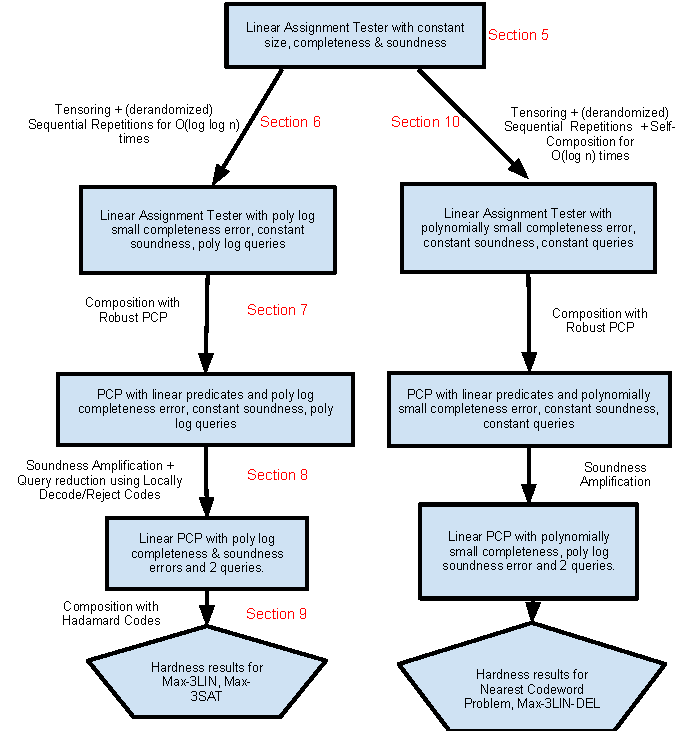
\includegraphics{Layout}
\caption{Layout of our Construction.}
\label{figure:layout}
\end{figure}

\newpage
%{\huge{Appendix}}

\section{Basic Assignment Tester} \label{section:basic} In this section, we
construct a verifier with a linear predicate and constant size.  In
what follows, we work with assignment testers. The notion of
assignment testers was pioneered by \cite{DR,BGHSV} and more recently
as Locally Decode and Reject Codes (LDRC) \cite{MR08} and as {\sf
  dPCP} by \cite{DH}.  Informally, an assignment tester not only needs
to accept a correct proof almost always but reject a purported proof
which is far from any valid proof. Note that this is a stronger
requirement to that of a PCP, where one aspires to verify only if
there exists an satisfying assignment to that instance of the problem.
We restrict ourselves to {\em linear} assignment testers. These are
assignment testers where every output circuit in $\Psi$ computes a
linear function over its variables.

\begin{definition}[Assignment Tester] \label{AT} An $(\rho,
  \delta)$-Assignment Tester is a reduction whose input is a Boolean
  constraint $\psi$ over a set of Boolean variables $X$. The output of
  the reduction is a system of constraints $\Psi$ over variables $X$
  and auxiliary variables $Y$ such that for every assignment $\pi: X
  \rightarrow \{0,1\}$,
\begin{itemize}
\item {\sf Completeness:} If $\pi$ satisfies $\psi$ then there exists
  an assignment $\tilde{\pi} : Y \rightarrow \{0,1\}$ such that $\pi
  \cup \tilde{\pi}$ satisfies at least $( 1 - \rho)$ fraction of
  the constraints in $\Psi$.
\item {\sf Soundness:} For every $\delta' < \delta$, if $\pi$ is
  $\delta'$-far from a satisfying assignment for $\psi$, then for
  every assignment $\tilde{\pi}: Y \rightarrow \{0,1\}$, at least
  $\Omega(\delta')$ of the constraints in $\Psi$ reject $\pi \cup
  \tilde{\pi}$.
\end{itemize}
\end{definition}


\paragraph{Standard Definitions.} We identify the {\em long code} of
${\bf x} \in \{\pm 1\}^n$ by $\LC$({\bf x}) $= \{ f({\bf x}) | f : [n]
\rightarrow \{\pm 1\} \}$. Informally, we evaluate {\bf x} on every
Boolean function on $n$ bits. We usually identify the domain of \LC \
with the Boolean hypercube $\{\pm 1\}^n$. We use the letters $f, g$
for points on the hypercube. We use $A, B$ and $\chi$ to denote
functions whose domain is in the hypercube. In particular, we consider
functions whose domain is an arbitrary set of size $n$. In this
application, this set is usually some $\{\pm 1\}^s$ such that $n =
2^s$.  For $\alpha \subset [n]$, define
\[
          \chi_\alpha : \{\pm 1\}^n \rightarrow \{\pm 1\},  \chi_\alpha(f) \triangleq \prod_{i\in \alpha}f(i)
\]

It is easy to check that the characters $\{\chi_\alpha\}_{\alpha
  \subseteq [n]}$ form an orthonormal basis for the space of functions
$\{A : \{\pm 1\}^n \rightarrow \mathbb{R}\}$, where inner product is
defined by $\langle A, B \rangle = \mathbb{E}_f[A(f) B(f)] =
2^{-n}\sum_fA(f)B(f)$. It follows that any function $A: \{\pm 1\}^n
\rightarrow \{\pm 1\}$ can be written as $A = \sum_\alpha
\hat{A}_\alpha \cdot \chi_\alpha$, where $\hat{A}_\alpha =\langle
A,\chi_\alpha \rangle$. 

\paragraph{The Long Code Test.}\label{LC} Let $A : \{ \pm 1\}^n \rightarrow \{\pm 1\}$ be
the purported long code of some fixed {\bf v}. We intend to test if
$A$ is infact The test picks two uniformly random vectors ${\bf x,y}
\in \{\pm1\}^W$ and then a vector ${\bf z} \in \{\pm1\}^W$ according
to the following distribution: for every coordinate $i \in [W]$, with
probability $1 - \rho$ we choose $z_i = 1$ and $z_i = -1$ otherwise.
It is useful to imagine ${\bf z}$ as a noise vector. The test accepts
iff $A({\bf x}) A({\bf y}) = A({\bf xyz})$. In other words, iff $z_w =
1$, which happens with probability $1 - \rho$. It follows from the
construction that the test accepts any valid long code encoding with
probability $1 - \rho$.

\begin{lemma}[H{\aa}stad's lemma \cite{Has97}]
If the test accepts with probability $1/2 + \delta$, then 
$\sum_\alpha \hat{f}^3_\alpha \cdot (1 - 2\rho)^{|\alpha|} \ge 2\alpha$.
\end{lemma}

\begin{corollary}
  If $f$ passes the long code test with probability with $1/2 +
  \delta$, then for $k = \frac{1}{2\rho}\log\frac{1}{\epsilon}$, there
  exists $\alpha$ with $|\alpha| \le k$ such that $\hat{f}_\alpha \ge
  2\delta - \epsilon$.
\end{corollary}

\begin{lemma}[Tester Lemma]\label{longcode}
  For every $\delta < 1/4$ there is a constant $\eta(\delta) > 0$,
  such that a table $A$ which is $\delta$-far from any valid long code
  encoding is rejected with probability $\ge \Omega(\delta)$.
\end{lemma}
\noindent {\em Proof.}  Assume that $A$ test passes with probability
$> 1 - \delta$. That is,
\begin{align*}
\	   \Pr \left [A\ \mbox{passes}\ \right]  &\ge 1 - \delta \\
& \implies  \exists k \le \eta,\  \mbox{such that} \ \hat{f}_k \ge 2 \cdot (1/2 -\delta ) - \epsilon \\
 &\implies  \exists \alpha \subset [n],  |\alpha|  \le k \  \mbox{s.t.}\  \chi_\alpha \  \mbox{is}\  \Omega(\delta')\mbox{-far}\ \mbox{from}\  A \\
 \end{align*}
 Note that $\chi_\alpha$ can be expressed as $\prod_{i \in \alpha}
 \chi_i$ and $|\alpha|$ is a constant.  Thus, any of the $\chi_i$'s
 agrees with $\chi_\alpha$ on at least $2^{-|\alpha|}$ fraction of the
 domain. Putting this in the context of agreement between $A$ and
 $\chi_i$: $\chi_i$ disagrees with $A$ on at least $1/2^{|\alpha|}
 \cdot \delta'$ fraction, which is essentially $\Omega(\delta)$. \qed

 \paragraph{Folding.} As done in \cite{BGS}, we fold the long code
 tables over true and the respective constraint $\psi$. This means
 that whenever the test needs to read $A[f]$, it reads $A[\psi \wedge
 f]$ instead. In addition, we fold over true which means for every
 pair $f$ and $-f$, we let $A$ specify only one and access the other
 via the identity $A[f] = - A[f]$. In short, we assume that $A[f] =
 A[f \wedge \psi]$ and $A[f] =- A[-f]$ for all $f$. It is well known
 that after folding $\hat{A}_\alpha = 0$ whenever $|\alpha|$ is even
 or there exists an $i$ in $\alpha$ for which $\psi(i) = 1$ (recall
 that $1$ corresponds to false).

 We are now ready to present the assignment tester needed for our
 construction. Let $\psi$ be a Boolean constraint over Boolean
 variables $x_1, x_2 \ldots x_s$. We describe an algorithm whose input
 is $\psi$ and whose output will be a system of linear equations
 satisfying the requirements of Definition \ref{AT}. 


 \noindent The tester seeks as input a satisfying assignment $\sigma$
 to $\psi$ and the $\LC(\sigma)$, $\LC(\sigma) \equiv A : L
 \rightarrow \{\pm 1\}$. Also, we assume that $A$ is folded over
 $\psi$. We can imagine $\LC(\sigma)$ as the set of auxilary variables
 used by the tester. We now describe the two kinds of constraints we
 place over these variables. Say, the tester gets two tables $\sigma$
 and $A$ as input.
	
\begin{enumerate}
\item {\sf Long Code Constraints:} The first set of constraints aims
  at testing if $A$ is indeed a valid long code encoding. It includes
  $3$ variable constraints derived from the {\em long code} test
  specified earlier. Specifically, we shall have one constraint per
  each coin toss of the long code test.

\item {\sf Consistency Constraints:} The second set of constraints
  include the following: For each choice of $i \in [s]$ and $f \in L$
  place a constraint that is satisfied iff $\sigma(x_i) = A(f) \oplus
  A(f \oplus e_i)$\footnote{$e_i$ is the vector of dimension $s$ with
    a $-1$ in $i$-th index and $1$ elsewhere.}. For the ease of
  argument, assume that are an equal number of constraints of each
  type\footnote{This can be easily achieved by placing multiple copies
    of the constraint of each type with appropiate multiplicity.}.
\end{enumerate}

\begin{lemma}[Assignment Tester] \label{Tester} For any $\rho > 0,
  \delta < 1/4$, the constraint system constructed above is a ($\rho,
  \delta$)-assignment tester for any Boolean function $\psi : [s]
  \rightarrow \{0,1\}$. Moreover, the output circuits of the
  assignment testers compute linear functions of their inputs.
\end{lemma}
\noindent {\em Proof.} Linearity of the constraints follows from
construction. We now analyze the parameters of the tester below
parameter by parameter.

\begin{itemize}

\item Completeness: For any good assignment that satisfies the
  constraint $\psi$, the second set of constraints are always
  satisfied. The only case where we reject a good proof is during the
  long code test and this happens with probability at most $1 - \rho$.

\item Soundness: Say, the tester gets $\sigma$ and $\pi$ as input and
  $\sigma$ is $\delta$-far from a satisfying assignment of $\psi$, we
  shall show that the tester rejects with probability at least
  $\Omega(\delta)$. Since $\pi$ was folded across $\psi$, $\pi$ is
  accepted by the long code constraint iff the assignment encoded by
  $\pi$ is a satisfying assignment to $\psi$. Since $\sigma$ is an
  unsatisfying assignment, if $\pi$ encoded $\sigma$, we would reject
  with probability greater than $\Omega(\delta)$. Thus, it must be
  that one of the following holds. (1). $\pi$ is a far from long code
  of $\sigma$. (2). $\pi$ is in fact a long code encoding. However,
  since $\pi$ was folded across $\psi$, we may assume that $\pi$
  encodes a satisfying assignment to $\psi$.

  In the former, it follows from Lemma \ref{longcode} that if $\pi$ is
  $\delta$-far from a valid long code table is rejected with
  probability greater than $\Omega(\delta)$ and by our construction
  these constraints constitute at least $\Omega(\delta)$-fraction of
  the total constraints. Thus, we reject any $\pi$ that is
  $\delta$-far from a valid long code encoding with probability at
  least $\Omega(\delta)$.

  In the latter, say $\pi$ encoded a satisfying assignment
  ${\sigma'}$. Since, $\sigma$ is $\delta$-far from a satisfying
  assignment, it must be that $\sigma$ is $\delta$-far from
  ${\sigma'}$. Hence, $Pr_i[\sigma(x_i) \ne \sigma'(x_i)] \ge
  \delta$. Thus, we have
\begin{equation}\label{equation}
   \Pr_{f \in L} \left[ \pi(f) \oplus \pi(f +e_i) = f(\sigma') \oplus (f \oplus e_i)(\sigma') \right] \ge 1 - 2\delta 
\end{equation}
Also, if $\sigma(x_i) \ne \sigma'(x_i)$, then $f(\sigma') \oplus (f
\oplus e_i)(\sigma') = \sigma'(x_i) \ne \sigma(x_i)$.  Hence, every
$f$ that satisifies Equation \eqref{equation} causes the corresponding
constraint constraint to reject. This implies that at least
$\Omega(\delta)$ of constraints of the second type are rejected. Thus,
in either case we reject the purported proof with probability at least
$\Omega(\delta)$.


 \eat{
\item Query Size: The tester picks at random a long code constraint or
  a consistency constraint. In either case, it makes $3$ queries.

\item Randomness: The tester uses $2 \cdot s$ bits of randomness.
}
\end{itemize}

\qed

We denote the {\sf size} of a linear tester by the $n$ and it refers
to the quantity $q \cdot m$, where $q$ is the number of queries made
by the tester and $m$ is the total number of equations in the
tester. Linear assignment testers cannot have perfect completeness.
For otherwise, one may use guassian elimination to figure out the if
there is an assignment that satisfies all the linear constraints and
reject if there isn't one. Hence, any linear tester is forced to have
a non-zero completeness error. Also, the soundness is always less than
$1/2$ as a random assignment satisfies at least $1/2$ of the equations
in $\eL$ in an expected sense (follows from the fact that the
equations are over ${GF}(2)$). As highlighted earlier, having low
completeness error becomes handy in several scenarios. We now
highlight on how we intend to use the tools we developed in the
previous section to achieve completeness amplification.


\section{Completeness Amplification}  \label{section:complete}

In this section, we employ tensoring to amplify the completeness of
the assignment tester we have built in Section \ref{section:basic}.
In what follows, we start with notations and a few observations that
will be useful to us in amplifying the completeness of the assignment
tester.\eat{ Let $\eL \equiv {\bf Ax} + {\bf y} = {\bf 0}$ denote the
  linear assignment tester given to us by Lemma \ref{Tester}. We now
  show that the d($\A$), d($\A$) $\equiv \min_{{\bf x} \ne {\bf 0}}
  {\bf Ax}$, is non-zero.

\begin{proposition}\label{longcodeisbest}
  Let $\eL \equiv {\bf Ax} + {\bf y} = {\bf 0}$ be the assignment
  tester obtained via Lemma \ref{Tester}. Then, for every ${\bf x_1}$
  and ${\bf x_2}$, ${\bf x_1} \ne {\bf x_2}$, the Hamming weight of
  ${\bf A} \cdot ({\bf x_1} + {\bf x_2})$ is a non-zero quantity. In
  other words, d($\A$) $> 0$.
\end{proposition}
\noindent {\em Proof.} To establish this, we consider the long code
constraints. Observe that the constants in the long code constraints
arise from the noise vector {\bf z}. Thus, modulo the noise vector the
long code constraints are over auxilary variables $\pi$ of the tester
and are the following: $\Pi$ = $\pi(i) + \pi(j) + \pi(i + j) \ \forall
\ i,j \in |\pi|$. Now, since ${\bf x_1} \ne {\bf x_2}$, they either
differ on exactly $0 < k \le |\pi|$ coordinates. ${\bf x_1}$ and ${\bf
  x_2}$ evaluate different on every equation in $\Pi$. In the latter,
say they disagree on $\pi({\bf 0})$, then they evaluate differently on
$\pi(\alpha) + \pi({\bf 0}) + \pi(\alpha + {\bf 0})$. If however they
agree on $\pi({\bf 0})$, then either they disagree only one coordinate
$\beta$ or on more than one coordinates. In the former, ${\bf x_1}$
and ${\bf x_2}$ disagree on $\pi(\beta) + \pi(\alpha) + \pi(\alpha +
\beta)$. \qed }

\begin{definition} Let ${\cal T}$ denote the assignment tester
  obtained via Lemma \ref{Tester} and $\psi : [s] \rightarrow \{0,1\}$
  denote the Boolean predicate being tested. For any proof $\Pi$
  provided to ${\cal T}$, we denote by $\Pi_\psi$ the assignment
  induced by $\Pi$ on the variables of $\psi$. Also, we denote by
  $\psi(\Pi_\psi)$ the evaluation of $\psi$ on $\Pi_\psi$.
\end{definition}

\begin{observation} \label{invariant} For any given proof $\Pi$ to
  assignment tester ${\cal T}$ to verify the satisfiability of $\psi$,
  $\Pi_\psi$ and $\Pi^{\otimes 2}_\psi$ are exaclty the same. More
  importantly, the distance of $\Pi_\psi$ to a satisfying assignment
  of $\psi$ remains uneffected by tensoring. The converse also holds.
\end{observation}
\noindent {\em Proof Sketch.} The converse follows from the fact that
we are extracting the assignment $\Psi_\psi$ from $\Pi$ from the
diagonal entries of $\Pi$.

In fact, the aforementioned observation can be extended to any
$\Pi^{\otimes k}$ and any $\Pi^{\otimes j}, \ 0 < j \le k$. We are now
ready to amplify the completeness of the basic assignment tester we
have constructed in Lemma \ref{Tester}.

\begin{lemma}[Tensored Assignment Tester] \label{tensortester} For any
  $\rho > 0, \delta < 1/4$, there is a ($\rho^2, \delta^2$)-assignment
  tester for any Boolean function $\psi : [s] \rightarrow
  \{0,1\}$. Moreover, the predicate of the assignment tester is
  linear.
\end{lemma}
\noindent {\em Proof.} We invoke Lemma \ref{Tester} to construct a
($\rho, \delta$)-assginment tester ${\cal T}$.  Let $\Pi$ denote proof
required by ${\cal T}$. We can now construct a ($\rho^2,
\delta^2$)-assginment tester ${\cal T}^{\otimes 2}$ as follows. The
proof required by ${\cal T}^{\otimes 2}$ will be ${\Pi}^{\otimes
  2}$. Thus, the new proof format will be $(\sigma \circ \pi)^{\otimes
  2}$ and the variables of $\psi$ will be $\{ \sigma_{ii}\}$ and the
rest will be auxilary variables of the new tester. The tests performed
by ${\cal T}^{\otimes 2}$ will be tensored tests of ${\cal T}$. In
other words, if the tests of ${\cal T}$ are $\eL$, then the tests of
${\cal T}^{\otimes 2}$ are linear equations in $\eL^{\otimes 2}$
(ref. Definition \ref{Tensoring}). We shall now analyze the parameters
of ${\cal T}^{\otimes 2}$.
\begin{itemize}
\item Completeness: In the good case, if there is a proof $\sigma
  \circ \pi$ which ${\cal T}$ accepts with probability at least $1 -
  \rho$. We invoke Proposition \ref{basic} to conclude that the
  probability that the verifier whose tests are ${\cal T}^{\otimes 2}$
  accepts $\left(\sigma \circ \pi\right)^{\otimes 2}$ is at least $1
  -$ UNSAT($\eL, \sigma \circ \pi$)$^2$, which is $1 - \rho^2$.

\item Soundness: We shall establish that for any purported proof
  $\Pi$, if $\Pi_\psi$ is $\delta^2$-far from a satisfying assignment
  to $\psi$, then ${\cal T}^{\otimes 2}$ rejects with probability at
  least $\Omega(\delta^2)$.  In order to establish this, we deal with
  the contrapositive of the claim.  Say, if $\Pi$ is accepted with
  probabilty $1 - \delta^2$, we shall show that $\Pi_\psi$ is not
  $\Omega(\delta^2)$-far to a satisfying assignment of $\psi$.

  Say, $\Pi$ is accepted with probability at least $1 - \delta'$, we
  can use Lemma \ref{converse} to infer that the diagonal vector of
  ${\Pi}$ gives us a proof which ${\cal T}$ accepts with probability
  at least $\alpha = 1 - \lfloor \frac{\delta'}{\delta}\rfloor$, where
  $\delta' < 1/16$. For the parameters that we have choosen, if
  $\delta' = \delta^2$ then $\alpha \simeq 1 - \Omega(\delta)$. In
  other words, if $\Pi$ has an acceptance probability of $1 -
  \delta^2$, then we can decode a proof $\pi$, which ${\cal T}$ would
  accept with probability $1 - \delta$. And from Lemma \ref{Tester},
  we know that if ${\cal T}$ accepts $\pi_\psi$ with probabilty at
  least $1 - \delta$, then it ain't $\Omega(\delta)$-far from a
  satisfying assignment of $\psi$.

  But, from Observation \ref{invariant} we can infer that $\Pi_\psi$
  is exactly same as $\pi_\psi$. Thus, if $\pi_\psi$ is not
  $\delta$-far from a satisfying assignment of $\psi$, so is
  $\Pi_\psi$. Also, by hypothesis, ${\cal T}^{\otimes 2}$ accepts
  $\Pi$ with probability $1 - \delta^2$. Hence, we can conclude that
  for every $\Pi$, if $\Pi$ is accepted with probability at least $1 -
  \delta^2$, then $\Pi_\psi$ is not $\Omega(\delta)$-far from a
  satisfying assignment. Since $\delta^2 < \delta$, it follows that if
  $\Pi_\psi$ is $\delta$-far from a string, it is trivially
  $\delta^2$-far. Therefore, the soundness of ${\cal T}^{\otimes 2}$
  holds.  
\item Query size: ${\cal T}^{\otimes 2}$ needs to make as many queries
  as the number of variables in an equation of $\eL^{\otimes 2}$. And
  this happens to be $q^2$.

\item Randomness: The randomness used by ${\cal T}^{\otimes 2}$ is
  $\log \eL^{\otimes 2}$, which is $2 \cdot \log \eL$. Thus, we double
  the randomness used whenever we tensor ${\cal T}$.
\end{itemize}
\qed \\

\noindent Notice that the above transformation preserves the linearity
of the tester. The downside of tensoring is that while it enhances the
completeness, it also destroys the soundness. Ideally, we would like
to improve the acceptance probability of the verifier in the good case
and leave the acceptance probability in the bad case unperturbed. Thus
to improve the soundness of the tester after the tensoring operation,
we resort to sequential repetition.

\paragraph{Soundness Amplification of the Tester.}
Sequential repetition of a Tester involves repeating the tests
sequentially with independent trails. For instance, performing
sequential repetition once would involve creating a new linear system
by picking every pair of equations in $\eL$ and then summing them up
to obtain a new linear system $\eL'$ whose size is twice the size of
$\eL$. This transformation converts a $(\rho, \delta)$-tester into a
$(2 \cdot \rho ,2 \cdot \delta)$-tester. In general, performing it
$\vartheta$ times on $(\rho , \delta)$-tester leaves us with a
$(\vartheta \cdot \rho, \vartheta \cdot \delta)$-tester.  However,
this operation does not preserve linearity. Thus, we resort to picking
${\cal O}(1)$ tests of the assignment tester and then, adding all
possible linear combinations of these tests to the create a new
assignment tester. The idea is that even if one the ${\cal O}(1)
equations$ are not satisfied by some assignment, half of the linear
combinations of these equations will also not be satisfied by the
assignment. To keep the size of the output assignment tester instance
small, we pseudo-randomly generate only ${\cal O}(n)$ of the $n^{{\cal
    O}(1)}$ possible ways to pick ${\cal O}(1)$ tests from $n$
tests. When given a $( \rho^2, \delta^2)$-assignment tester as an
input, we wish to produce an $(\rho^2, \delta)$-assignment tester as
the output.

We can achieve this via randoms walks on expanders or essentially any
one of its variants like samplers. We aim to achieve the following. We
wish to take a random walk on a expander so that the probablilty of
visiting a subset containing $\delta$ fraction of the vertices is at
least $2 \cdot \delta$.

A {\em walk of length l} in a graph $G = (V,E)$ is a sequence $v_0,
\ldots v_l$ of vertices of $G$, where for $1 \le i \le l$,
$v_{i-1}v_i$ is an edge in $G$. By a simple calculation, the total
number of walks of length $l$ in any $d$-regular graph is exactly
$|V|\cdot d^l$. Suppose there is a subset $C$ of $V$, we wish to bound
the number of walks that do not contain a vertex from $C$. If $G$
happens to be disconnected, it may happen that a constant fraction of
them avoid $C$. However, Ajtai, Koml$\grave{o}$s and
Szemr$\grave{e}$di (1987) show that if all the eigen values of $G$,
with the exception of the largest are small, then there are far fewer
of walks avoiding $C$. We now state their result.

\begin{theorem} \label{walks}
  Let $G = (V,E)$ be a $d$-regular graph on $n$ vertices, and suppose
  that each of its eigenvalues but the first one is at most
  $\lambda$. Let $C$ be a set of $cn$ vertices of $G$. Then, for
  every, the number of walks of length $l$ in $G$ that avoid $C$ does
  not exceed $(1 - c)\cdot n \cdot ((1 - c) \cdot d + c \cdot
  \lambda)^l$.
\end{theorem}

Now, a {\em randomly chosen walk} of length $l$ in $G$ chosen
according to a uniform distribution among all walks of that length.
If $G$ is regular, then such a walk can be chosen by choosing its
starting point $v_0$ uniformly at random and then picking the next
vertex of the walk among the $d$ neighbours of $v_0$ uniformly at
random.

\begin{corollary}
  Let $G = (V,E), d, n, \lambda, C$ and $c$ be as in Theorem
  \ref{walks} and suppose 
\[
(1 - c)\cdot d + c \cdot \lambda \ \le \ \frac{d}{\sqrt{2}}
\]
Then, for every $l$, the probability that a randomly chosen walk of
length $l$ in $G$ avoids $C$ is at most $2^{{-l}/{2}}$.
\end{corollary}




\eat{In this work, we make use of a samplers based approach. Samplers
  are pseudo-random objects that are extremely useful in simulating a
  random walk or drawing random samples. In what follows, we denote
  the neighbours of a vertex $u$ in a graph by $\Gamma(u)$.

\begin{definition}[Samplers]
  A bipartite graph $H = (A,B,E)$ is said to be an $(\epsilon,
  \gamma)$-sampler if for every subset $S \subseteq A$,
\[
  \Pr_{b \in B}\left[ \frac{|\Gamma(b) \cap S|}{|\Gamma(b)|} > \frac{|S|}{|A|} + \epsilon \right] \le \gamma
\]
\end{definition}

In other words, neighbourhoods of most vertices $b$ behave like a
random sample of $A$, in the sense that that their density within any
fixed $S$ is close to what is expected.  The following article
\cite{Sample} by Oded Goldreich is an excellent exposition on
samplers, their constructions and applications.

\begin{theorem}\cite{Sample}\label{sample} There exists a polynomial 
  time algorithm that, given an integer $n$ and a parameter $\epsilon
  > 0$, outputs an $(\epsilon, \gamma)$-sampler with $|A| = |B| = n$
  and the right degree $4/\epsilon^4$. Moreover, the randomness used
  by the algorithm is bounded by $\log n + {\cal O}(\log 1/\epsilon )
  + {\cal O}(\log  1/\gamma)$.
\end{theorem}
}
\begin{lemma}[Soundness Amplification] \label{boosting} There is
  universal constant $\vartheta$, such that every ($\rho^2,
  \delta^2$)-assignment tester for a Boolean predicate $\psi$ over
  variable set $\sigma$ can be amplified to a $(\vartheta \cdot
  \rho^2, {\delta})$-assginment tester. Moreover, the new tester still
  has a linear predicate.
\end{lemma}
\noindent {\em Proof.} Let us denote the $(\rho^2,
\delta^2)$-assignment tester by $V$ and the tests performed by $V$
with $\eL$. Roughly, our approach will be to design a new assignment
tester $V'$ whose tests are the sum of $\vartheta$ tests of the old
verifier $V$, each of which is chosen independently at random. Thus,
$\eL' = \{ \phi_1 \oplus \phi_2 \ldots \oplus \phi_\vartheta : \phi_i
\in \eL \ \ \forall \ i \ \in [\vartheta]\}$. We fix $\vartheta$ to be
the length of random that one must take on an exapnder so that the
probability we hit a $\delta$ fraction of the tests is at least $2
\cdot \delta$. It follows that for an appropiate choice of expander
this can set to some constant less than $5$.  Note that even though
the tests of $V'$ are different from $V$, both of them expect the same
proof as in Lemma \ref{Tester}. We now establish that $V'$ is in fact
a $(\vartheta \cdot \rho^2, {\delta})$-tester.
\begin{itemize}
\item Completeness: In the good case, $V$ rejects a valid proof
  $\sigma \circ \pi$ with probability at most $\rho$. Now by the union
  bound, the probability that $V'$ rejects it is at most $\vartheta
  \cdot \rho^2$.
 
\item Soundness: Say, we are given an assignment tester $V$ that
  rejects any proof $\Pi$ such that if $\Pi_\psi$ (projection of $\Pi$
  on the variable set $\sigma$) is $\delta$-far from a satisfying
  assignment of $\psi$, it is rejected with probability at least
  $\Omega(\delta)$.  The claim we make is that the assignment tester
  $V'$ will get reject any $\Pi$ such that $\Pi_\psi$ is $\delta$-far
  from a satisfying assignment to $\psi$ with probabilty at least
  $\Omega({\delta})$. Consider the scenario that $V$ rejects a proof
  that is $\delta$-far from a satisfying assignment of $\psi$.  It
  follows from our parameters that probability we do not hit the bad
  set is at most $\delta$ and hence, the soundness condition holds.

\item Query size: The arity of the equations in $\eL'$ is $\vartheta
  \cdot q$, where $q$ is the arity of $V$.

\item Randomness: Since, we are drawing $\vartheta$ independent
  samples from $\eL$, we would be needing $\vartheta \cdot r_V$, where
  $r_V$ is the randomness used by $V$.
\end{itemize}
 \qed

\eat{
\begin{lemma}[Derandomization Lemma] \label{derandomize} For every $\rho
  > 0, \delta < 1/4$, $\vartheta < \min(1/\rho,1/\delta)$ and $\vartheta$
  sequential repetitons of every ($\rho, \delta$)-assignment tester can be achieved using
  only $r_v + {\cal O}(\log \vartheta)$ random bits.
\end{lemma}
\noindent{\em Proof.} Follows by invoking Theorem \ref{sample} to
construct a $(\epsilon, \gamma)$-sampler and use it instead of
sampling $\vartheta$ tests of verifier at random. Specifically, set $n
= 2^{r_v}$, $\gamma = 1- \vartheta \cdot \delta$, $\epsilon$ will be
fixed latter.  We now establish that this process actually simulates
sequential repetition in a randomness efficient way. During sequential
repetition, we wish to test independent samples of the verifier's
test. Consider the soundness case, here we would like to sample one of
the constraints that fail the verifier's test. Say, a set $S$ of the
tests fail. So, we would like to hit one of these tests. In a
sequential repetition, the probability that we hit this set is
$\vartheta \cdot \frac{|S|}{|A|}$.

We aim to achieve the aforementioned claims via a sampler. For a
sampler to have failed us, it must be that the vertex $b$ on the right
must have had all its neighbours in the complement (denote this set by
$\overline{S}$) of $S$ that we wanted to hit. And, the probability
that this would happen is
\begin{align*}
  \Pr_{b \in B}\left[ \frac{|\Gamma(b) \cap \overline{S}|}{|\Gamma(b)|} = 1 \right] 
  = \Pr_{b \in B}\left[ \frac{|\Gamma(b) \cap \overline{S}|}{|\Gamma(b)|} = 1 - \frac{|S|}{|A|} + \frac{|S|}{|A|} \right] 
  =  \Pr_{b \in B}\left[ \frac{|\Gamma(b) \cap \overline{S}|}{|\Gamma(b)|} =  \frac{|\overline{S}|}{|A|} +  \frac{|S|}{|A|} \right] 
%  =& \Pr_{b \in B}\left[ \frac{|\Gamma(b) \cap \overline{S}|}{|\Gamma(b)|} =  \frac{|\overline{S}|}{|A|} +  \frac{|S|}{|A|} \right] \\
  \end{align*}
We invoke Theorem \ref{sample} for $\epsilon \in (0, \frac{|S|}{|A|}]$.  
\begin{align*}
  \Pr_{b \in B}\left[ \frac{|\Gamma(b) \cap
      \overline{S}|}{|\Gamma(b)|} > \frac{|\overline{S}|}{|A|} +
    \epsilon \right] \le 1 - \vartheta \cdot \delta \implies \Pr_{b \in
    B}\left[ \frac{|\Gamma(b) \cap {S}|}{|\Gamma(b)|} > \epsilon
  \right] >  \vartheta \cdot \delta
\end{align*}

Hence, the completeness and soundness of this new assignment tester is
$\vartheta \cdot \rho$ and ${\vartheta} \cdot \delta$
respectively. This is essentially what we achieve with $\vartheta$
sequential repetitions as in Lemma \ref{boosting} but with a larger
query complexity $1/\epsilon^4$. If $\epsilon = \Theta(1/\vartheta)$,
then the query complexity happens to be ${\cal O}(\vartheta^4)$. The
bounds on randomness follows from Theorem \ref{sample}.
\qed\\
}
\begin{corollary}[Tensoring + Repetition]\label{iterate}
  For every $\rho > 0, \delta < 1/4$, there is an absolute constant
  $\vartheta$, given a $(\rho, \delta)$-assignment tester that uses
  $r_v$ random bits to make $q$ queries, we can construct a ${\cal
    O}\left(\rho^2 \cdot \vartheta , {\delta}\right)$-assignment
  tester. The new assginment tester uses $r_v \cdot \vartheta)$ random
  bits and makes ${\cal O}(\vartheta \cdot q^2)$ queries.
\end{corollary}
\noindent {\em Proof.} Say, the $(\rho, \delta)$-assignment tester $T$
requires a proof $\Pi$. Since, we start with the assignment tester
given by Lemma \ref{Tester}, $\Pi = \sigma \circ \pi$, where $\sigma$
are the variables of the Boolean predicate being verified and $\pi$ is
the auxilary variables introduced by the assignment tester. Our new
tester requires the proof $(\sigma \circ \pi)^{\otimes 2}$ and its
tests are invoking Lemma \ref{tensortester} to obtain the tensored
tests of the input assignment tester, and then followed by Lemma
\ref{boosting} with parameters $\delta = 16/100$, $\vartheta = 5$ and
$\rho = 1/\left(2 \cdot \vartheta\right)$ .  We now argue the
completeness and soundness of the newly constructed assignment tester
$N$.
\begin{itemize}
\item {\em Completeness:} In the good case, if we have a proof that
  the input assignment tester $T$ accepts with probability $1 - \rho$,
  we can use Proposition \ref{basic} to claim that after invoking
  Lemma \ref{tensortester} on $T$, we have a completeness of $1-
  \rho^2$. Now, after the application of Lemma \ref{boosting} it
  follows from our parameters that the completeness of $1 - {\cal
    O}(\rho^2)$.
\item {\em Soundness:} Say, the newly constructed assignment tester
  $N$ is given a purported proof $\Pi$ such that $\Pi_\sigma$ (denotes
  the assignment induced on $\sigma$ by $\Pi$) is $\delta$-far from a
  satisfying assignment to $\psi$, we will establish that it is
  rejected with probability at least $\Omega(\delta)$.  One important
  inference from Observation \ref{invariant} is that the neither
  tensoring nor sequential repetitions, change the assignment to
  $\sigma$ and hence, its distance to a satisfying assignment of
  $\psi$. This if the input assignment tester has the soundness for
  $\delta < 1/4$, we can invoke the soundness arguments of Lemma
  \ref{tensortester} and \ref{boosting} to infer that soundness
  condition holds.
\end{itemize}
\qed

\begin{table}\label{roundup}
%\begin{table}
\centering
\begin{tabular}{|l|c|c|c|}
\hline
%\ & & \\
{\em Parameters}  &{ Tensoring} & {\parbox{0.85in}{Repetitions}} & \parbox{0.7in}{After $k$\\ Iterations}\\
	\hline
%\ &  & \\ 
        \hline
        {\tt Completeness} & $\rho^2$ & ${\cal O}\left(\vartheta' \cdot \rho^2\right)$  &  ${\cal O}(\vartheta' \cdot \rho^{k + 1})$ \\  
        {\tt Soundness} &   $\delta^2$ & $\delta$&  $\delta$ \\
        {\tt Queries} &   $q^2$ & $\vartheta\cdot q^2$ & $\vartheta^{ \cdot (k + 1)} \cdot  q^{k} $ \\
        {\tt Alphabet}&    $\{0,1\}$ & $\{0,1\}$ & $\{0,1\}$ \\
        \hline
\end{tabular} %\caption{Parameters after one iteration} \label{1round}
  \caption{Parameters of a ($\rho, \delta$)-assignment tester after various operations.}
\end{table}


\begin{lemma}[Completness Amplification Lemma]\label{Camplify}
  For every $\rho > 0, \delta < 1/4$, given a $(\rho,
  \delta)$-assignment tester with query complexity $\q = {\cal O}(1)$
  of size $2^{r_v}$, one can construct a $({\cal
    O}(\rho^k),\delta')$-assignment tester with query complexity $\q$,
  $\q = 1/\rho^{k'}$, in time polynomial in $2^{ k \cdot \left(r_v +
      {\cal O}\left(\log \vartheta\right)\right)}$.
\end{lemma}
\noindent{\em Proof.} Say we have a ($\rho, \delta$)-assignment tester
that verifies a Boolean predicate $\psi$ using a proof over variables
of $\psi$ (call them $\sigma$) and auxilary variables $\pi$. Our
$({\cal O}(\rho^k),\delta')$-assignment tester uses the proof ($\sigma
\circ \pi$)$^{\otimes k}$. The tests are tensored tests of Lemma
\ref{iterate}. Specifically, the tests new assignment tester are the
tests of lemma \ref{iterate} tensored with itself $k$ times.

However, we would like to iteratively apply the output of Lemma
\ref{iterate} upon on itself. This makes it easier to apply the tools
that we have build thus far.  The first observation we make is that
the after a $(\rho, \delta)$-tester, of size $n$, under goes $r$
recursive iterations of the Tensoring followed by $\sigma$ rounds of
sequential repetition, the size of the resulting tester is
$n^{2^{2^{r-1}}}$. This can be verified once we observe that we are
squaring the size of the input instance in every iteration. By
invoking Corollary \ref{iterate}, we infer that the completeness error
is also squared in each iteration. Hence after $r$ iterations, the new
error parameter is $\rho^{2^{2^{r-1}}}$. However, the soundness of the
tester remains uneffected. With this background, the Lemma follows by
setting $ r = \log \log k$. Notice that the proof required by this
recursive construction is same as that of the iterative assignment
tester constructed in previous paragraph.  The new proof will be
$(\sigma \circ \pi)^{\otimes k}$. Also, note that while the auxilary
variables blow up in every step, the variables of the Boolean
predicate that we are checking remain the same. The parameters are
summarized in Table \ref{roundup}.

\begin{itemize}
\item {\em Completeness:} It is by far the easier case to argue. Say,
  a $(\rho, \delta)$-assignment tester is given to us that enables us
  to verify a Boolean predicate using a proof $\Pi$. Then by Corollary
  \ref{iterate}, we have a new assignment tester which has the square
  of the completeness error after a single iteration. It follows that
  after $\log \log k$ iterations, we end up with a completeness error
  of ${\rho^k}$.

\item {\em Soundness:} Say that the $({\cal
    O}(\rho^k),\delta')$-assignment tester is given access to a
  purported proof $\Pi$, we need to show that the if the proof
  $\Pi_{\sigma}$ (denotes the projection of $\Pi$ on the variables of
  $\psi$) is $\delta'$-far to a satisfying proof of the Boolean
  predicate, the tester rejects with probability at least
  $\Omega(\delta)$. We show this property holds after each iteration
  and hence, the newly constructed assignment tester via this process
  always has the soundness condition. We begin by defining the
  projection of a proof on $\sigma$.  We denote by $\Pi_\sigma$ the
  assignment which $\Pi$ makes to the variables in $\sigma$.

  The approach is simple. We give a proof by induction on the number
  of iterations. The assignment tester produced after the first
  iterate is sound by Corollary \ref{iterate}. Assume that the
  assignment tester produced after $i$-th iterations is sound. We now
  show that the assignment tester produced after ($i+1$)-th iteration
  is also sound.  By assumption, the assignment tester at the $i$-th
  level has the soundness property, it now follows from Corollary
  \ref{iterate} that the soundness holds even after $(i+1)$-th
  iteration.

\item {\em Queries:} We again invoke Corollary \ref{iterate} to
  concude that the number of queries increase fourth power in
  $\vartheta$. Since the basic tester of Lemma \ref{Tester} made $\q =
  {\cal O}$(1) queries, after $\log \log k$ iterations we would have a
  query complexity of $\q^{k} \simeq 1/\rho^{k'}$.

\item {\em Randomness:} In every tensoring operation,
  we square the randomness (ref. Lemma \ref{tensortester}. Thus, the {\em
  randomness} of the tester after $r$ iterations is $k \cdot (r_v
  + {\cal O}(\log \vartheta))$, where $r_v$ is the
randomness used by the ($\rho, \delta$)-tester of Lemma \ref{Tester}. 

\item {\em Alphabet:} The alphabet of the tester obtained via Lemma \ref{Tester} 
has an alphabet $\{ 0,1\}$ and it remains unchanged during the application of Lemma \ref{iterate}.
\end{itemize}
\qed



